%%%%%%%%%%
\begin{frame}
    \centering
    \only<1>{%
        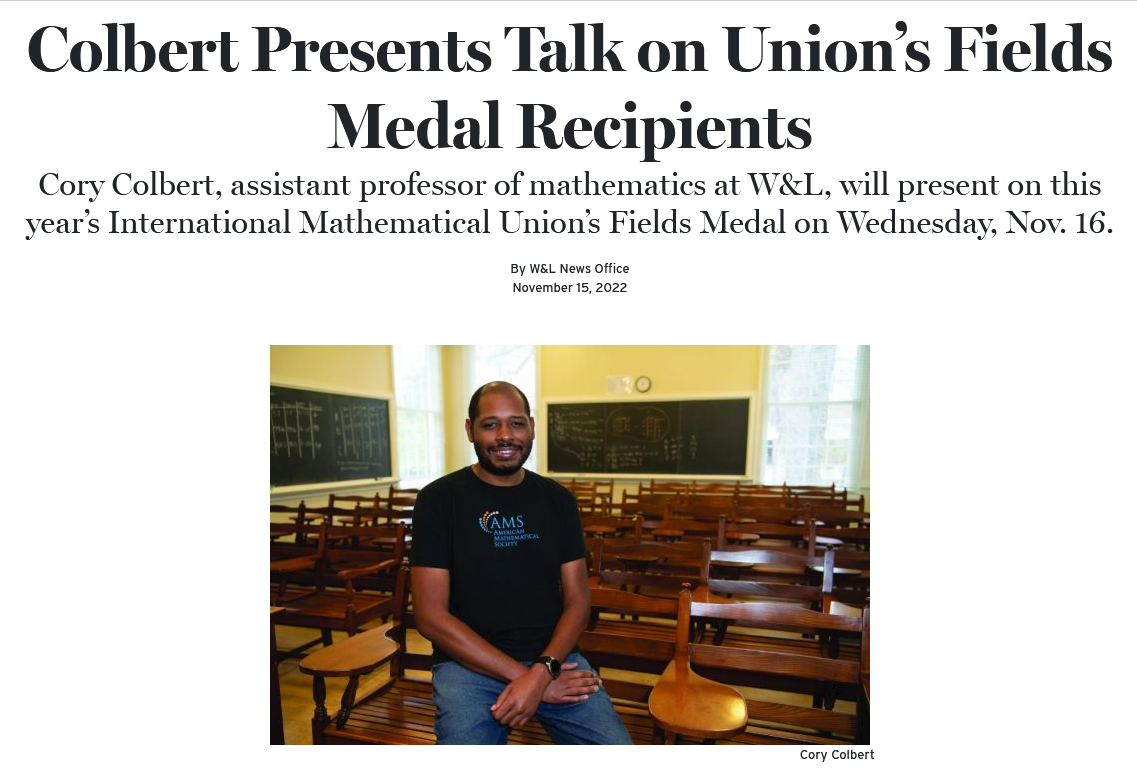
\includegraphics[width=0.85\textwidth]{./images_women_in_IT/colbert_math.png}
        % \caption{This is an example caption.}
    }
    \only<2>{%
        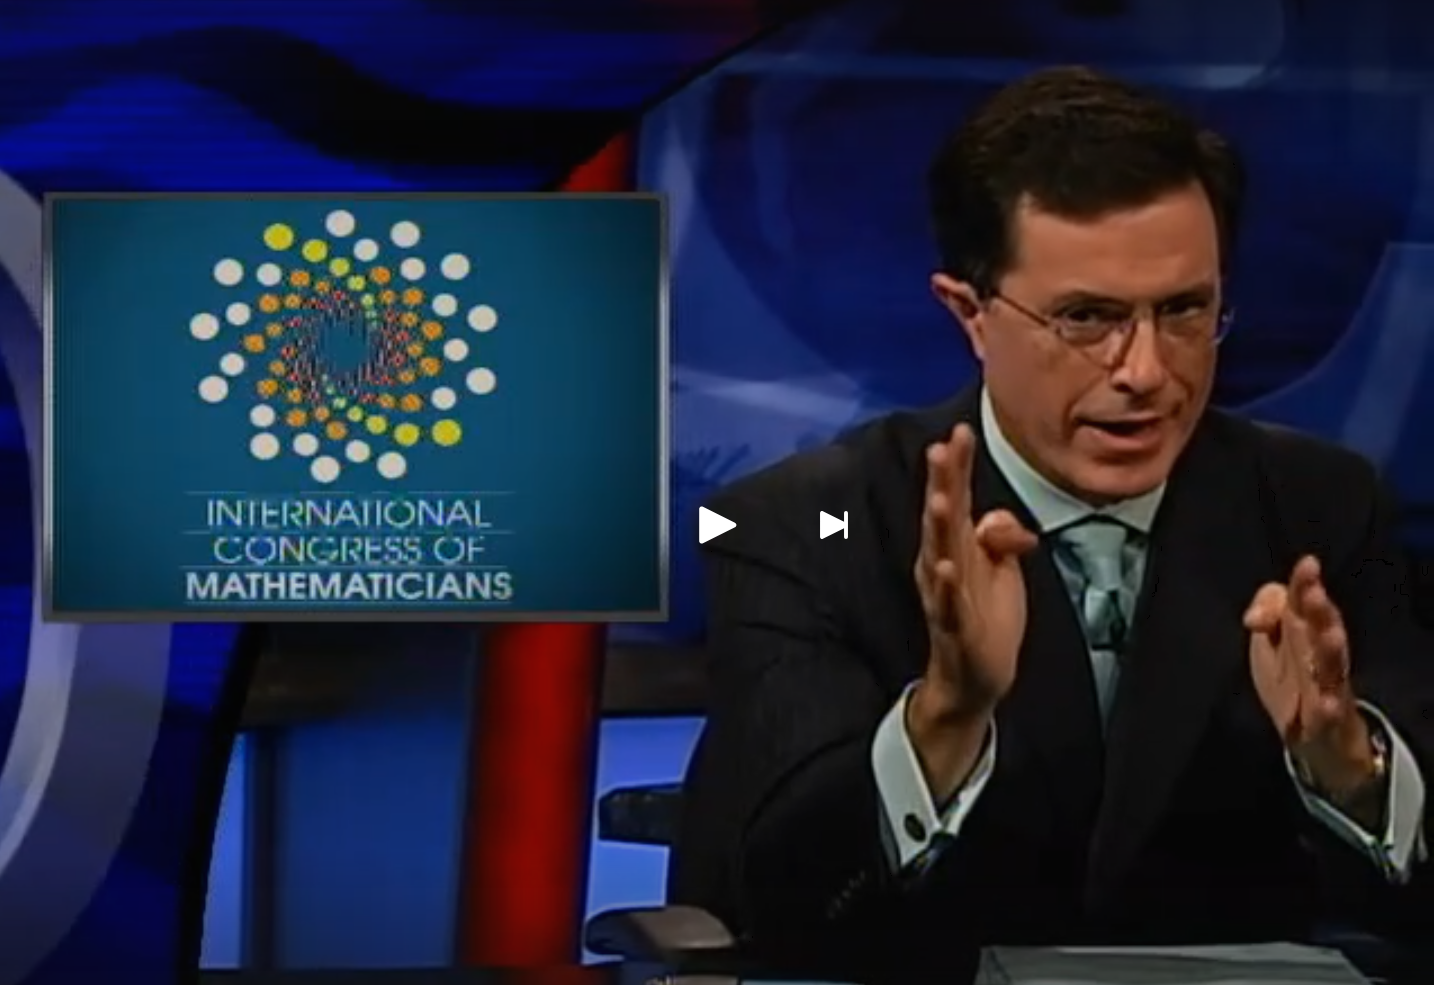
\includegraphics[width=0.75\textwidth]{./images_women_in_IT/stephen_colbert.png}
        \\ \href{https://www.dailymotion.com/video/x7yrghr}{Colbert on the Fields Medal.}
    }
\end{frame}

\begin{frame}{}
    \begin{columns}
        \begin{column}{.65\textwidth}
            \Huge \textbf{What is this stuff?}
            \begin{itemize}
                \item<2->Proof? 
                \item<3->Conjecture?
                \item<4->Weird Stuff with a bunny?
            \end{itemize}
        \end{column}
    \end{columns}
\end{frame}

\begin{frame}
    \centering
    \vfill
    \tikzset{%
        node/.style={draw, align=center, minimum width=2.5cm, minimum height=1cm, text width =2.5cm},
        circ/.style={node, circle, minimum height=1.2cm, text width =2.5cm},
        oval/.style={node, ellipse, minimum height=1.2cm, text width =2.5cm},
        >={Latex[length=3mm]},
        arrow/.style={->, thick}
    }

    \begin{tikzpicture}[scale=.5,node distance=1.6cm]
        % Nodes
        \node[oval, fill=blue!25]   (start) {\small Spot patterns, connect ideas, explore, ...};
        \node[circ, fill=red!25, right=of start, visible on=<2->] (a) {\small Define, structure, abstract, conjecture, ...};
        \node[oval, fill=green!25, right=of a, visible on=<3->] (b) {\small Formalize, communicate, share, ...};
        \node[circ, fill=yellow!75, below =1cm of a, visible on=<4->] (d) {Understand\\ (hard things)};
        \node[circ, fill=yellow!60!red, below= of start, visible on=<7->] (end) {\small "Real-world"\\ tools};

        % Arrows
        \draw<2->[arrow] (start) -- (a);
        \draw<3->[arrow] (a) -- (b);
        \draw<4->[arrow] (b) |- (d);
        \draw<5>[arrow] (d) -| (start);
        \draw<7>[arrow] (d) -- (end);
        \draw<7>[arrow] (end) -- (start);
    \end{tikzpicture}
    \onslide<6->{The language of this process is "proof," and logic is its grammar.}
    \vfill
\end{frame}

\begin{frame}
    \only<1>{%
        \centering
        \vfill
        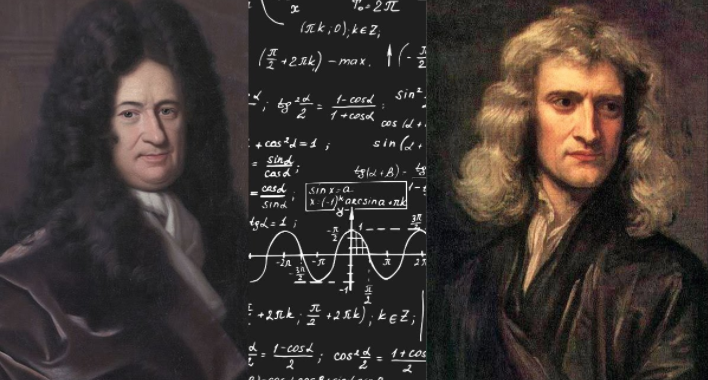
\includegraphics[width=0.85\textwidth]{./images_women_in_IT/newton_leibniz_calculus.png}
        % \caption{This is an example caption.}
    }
    \only<2->{%
            \vfill
            \textit{“I have never done anything ‘useful’. 
            No discovery of mine has made, or is likely to make, directly or indirectly, for good or ill, 
            the least difference to the amenity of the world.”} \\
            \hfill -G. H. Hardy (number theory) 1877–1947
    }
    \\ \vspace{30pt}
    \only<3->{%
            \textit{“Vector analysis is interesting, but it will never have any practical application.”}\\
            \hfill -William Thomson (Lord Kelvin) 1824-1907
    }
    \vfill
\end{frame}